%% LyX 2.4.4 created this file.  For more info, see https://www.lyx.org/.
%% Do not edit unless you really know what you are doing.
\documentclass[english,t]{beamer}
\usepackage{mathptmx}
\usepackage[T1]{fontenc}
\usepackage[latin9]{inputenc}
\usepackage{amssymb}
\usepackage{cancel}
\usepackage{wasysym}

\makeatletter
%%%%%%%%%%%%%%%%%%%%%%%%%%%%%% Textclass specific LaTeX commands.
% this default might be overridden by plain title style
\newcommand\makebeamertitle{\frame{\maketitle}}%
% (ERT) argument for the TOC
\AtBeginDocument{%
  \let\origtableofcontents=\tableofcontents
  \def\tableofcontents{\@ifnextchar[{\origtableofcontents}{\gobbletableofcontents}}
  \def\gobbletableofcontents#1{\origtableofcontents}
}

%%%%%%%%%%%%%%%%%%%%%%%%%%%%%% User specified LaTeX commands.
\usetheme{Warsaw}
% or ...

\setbeamercovered{transparent}
% or whatever (possibly just delete it)
\setbeamercovered{invisible} %makes overlays invisible

%gets rid of navigation symbols
\setbeamertemplate{navigation symbols}{}

%\usepackage{hyperref}
%\usepackage[usenames,dvipsnames,table]{xcolor} %adds additional color options
\definecolor{links}{HTML}{2A1B81}
%\hypersetup{colorlinks,linkcolor=blue,urlcolor=links}

\usepackage{multicol}

\usepackage{tikz}
\usetikzlibrary{calc}
\usetikzlibrary{plotmarks}
\usetikzlibrary{shapes}
\usepackage{pgfplots}
\pgfplotsset{compat=newest}

\usepackage{forest} %%for tree diagram

\usepackage{calc}
\usepackage[nomessages]{fp}

%\usepackage{advdate}    % Advancing/saving dates
\usepackage{datetime}   % Dates formatting
%\usepackage{datenumber} % Counters for dates

\usepackage[super]{nth}

\usepackage{etex}

\usepackage[outline]{contour}  %allows text halos
\contourlength{1pt} %sets halo width
%%example: \node at (0.75,0.5) {\contour{white}{\Large Text!}};
%%example:  \node [fill=white,inner sep=1pt] at (2.25,0.5) {\Large 			Text!};
%%example:  \node [fill=white,rounded corners=2pt,inner sep=1pt] at 			(3.75,0.5) {\Large Text!};

%%%%%%%%%%%%%%%%%%%%%%%%%%%
\def\formatdateny{\csname noyear\languagename\expandafter\endcsname\formatdate}
\def\noyearenglish#1, \the\@year{#1}
\let\noyearamerican\noyearenglish
\let\noyearbritish\noyearenglish

%%allows uncover with forest diagrams
\tikzset{
    invisible/.style={opacity=0,text opacity=0},
    visible on/.style={alt=#1{}{invisible}},
    alt/.code args={<#1>#2#3}{%
      \alt<#1>{\pgfkeysalso{#2}}{\pgfkeysalso{#3}} % \pgfkeysalso doesn't change the path
    },
}
\forestset{
  visible on/.style={
    for tree={
      /tikz/visible on={#1},
      edge={/tikz/visible on={#1}}}}}

%%%redefines column alignment to match vertically
%\define@key{beamerframe}{t}[true]{% top
  %\beamer@frametopskip=.2cm plus .5\paperheight\relax%
  %\beamer@framebottomskip=0pt plus 1fill\relax%
 % \beamer@frametopskipautobreak=\beamer@frametopskip\relax%
  %\beamer@framebottomskipautobreak=\beamer@framebottomskip\relax%
  %\def\beamer@initfirstlineunskip{}%
%}

%%provides pdf with 4 slides per page; don't forget to add 'handout' to remove overlays
%\usepackage{pgfpages}
%\pgfpagesuselayout{4 on 1}[a4paper, landscape, border shrink=7mm]
%\pgfpageslogicalpageoptions{1}{border code=\pgfusepath{stroke}}
%\pgfpageslogicalpageoptions{2}{border code=\pgfusepath{stroke}}
%\pgfpageslogicalpageoptions{3}{border code=\pgfusepath{stroke}}
%\pgfpageslogicalpageoptions{4}{border code=\pgfusepath{stroke}}
%%%Don't forget to add 'handout'

\makeatother

\usepackage{babel}
\begin{document}
\newcommand{\xmax}{2000}
\newcommand{\xmin}{0}
\newcommand{\xstep}{0} %must be xmin+n
\newcommand{\ymax}{500}
\newcommand{\ymin}{0}
\newcommand{\ystep}{0} %must be ymin+n

\newcounter{countEx} \setcounter{countEx}{0}
\newcounter{countProb} \setcounter{countProb}{0}
\resetcounteronoverlays{countEx} \resetcounteronoverlays{countProb}

\newcommand{\ex}[3]{
	\addtocounter{countEx}{1}
	\only<#1-#2>{\begin{exampleblock} {Example \chNum.\secNum.\arabic{countEx}.} #3	\end{exampleblock}}
}

\newcommand{\prob}[4]{
	\addtocounter{countProb}{1}
	\only<#1-#2>{\begin{exampleblock} {Problem  \chNum.\secNum.\arabic{countProb}.\,#3} #4	\end{exampleblock}}
}

\newcommand{\yline}[4]{
	(#2 - #4)/(#1 - #3)*(x - #1) + #2
}

\beamerdefaultoverlayspecification{<+->}

%%%%Chapter and Section numbers%%%%%
\newcommand{\chNum}{1}
\newcommand{\secNum}{1}
\newcommand{\secTitle}{Deductive VS Inductive Reasoning}

\title[Section \chNum.\secNum: \secTitle]{Section \chNum.\secNum: \secTitle}

\subtitle{Finite Mathematics~~MTH 107~~Fall 2014}

\author{Dr.\,James Ashe}

\titlegraphic{\includegraphics[height=2.75cm]{/home/jim/JamesAshe/MHU/images/MarsHilUniversityLogo-Virtical.png}}

\date{\formatdate{10}{9}{2014} and \formatdate{3}{9}{2014}}

\institute{Mars Hill University}

\makebeamertitle 
\begin{frame}{}

\begin{columns}


\column{5.5cm}
\begin{block}{Deductive Reasoning}
Reasoning from statements/assumptions to reach a logically \emph{certain}
conclusion.

\begin{itemize}
\item <2->Applying a general rule to a specific instance.
\item <6->\emph{Correct} premises give correct conclusions. 
\end{itemize}
\end{block}
\only<3-5>{
\begin{exampleblock}{Example Argument}

\begin{enumerate}
\item <3->[1.]All men are mortal.
\item <4->[2.]Socrates is a man.
\item <5->[]Therefore, Socrates is mortal.
\end{enumerate}
\end{exampleblock}
}

\only<6->{
\begin{exampleblock}{Example Argument}

\begin{enumerate}
\item <7->[1.]The area of a triangle is $\frac{1}{2}b\cdot h$.
\item <8->[2.]Triangle $T$ has a base of $3$ and height of $4$.
\item <9->[$\Rightarrow$]Therefore, the area of $T$ is $6$.
\end{enumerate}
\end{exampleblock}
}

\column{5.5cm}
\begin{block}<10->{Inductive Reasoning}
Reasoning in which the premises supply \emph{strong evidence }for
a conclusion.

\begin{itemize}
\item <11->Using specific cases to make a general statement. 
\item <15->Conclusion is \emph{not} necessarily correct.
\end{itemize}
\end{block}
\only<12-15>{
\begin{exampleblock}{Example Argument}

\begin{enumerate}
\item <13->Socrates drank milk and got sick.
\item <14->Socrates ate ice cream and got sick.
\item <15->[$\Rightarrow$]Therefore, Socrates is lactose intolerant.
\end{enumerate}
\end{exampleblock}
}

\only<16->{
\begin{exampleblock}{Example}

\begin{enumerate}
\item <17->[1.]All known life requires water.
\item <18->[]Therefore, life will only be found on planets with water.
\end{enumerate}
\end{exampleblock}
}
\end{columns}
\end{frame}

\begin{frame}{Valid/Invalid Arguments}

\vspace{-.5cm}
\begin{columns}


\column{5.5cm}
\begin{block}{Invalid Argument}
A deductive argument is \emph{invalid} if the premises are met, but
the conclusion does \emph{not necessarily} follow.

\begin{itemize}
\item <2->Use a Venn diagram.
\item <10->Correct conclusion $\nRightarrow$ valid argument.
\end{itemize}
\end{block}
\only<3-7>{
\begin{exampleblock}{Example}

\begin{enumerate}
\item [1.]<3->All presidents are men.
\item [2.]<5->Dr.\,Ashe is a man.
\item <6->[$\Rightarrow$]Therefore, Dr.Ashe is a US president.
\end{enumerate}
\end{exampleblock}
}

\only<8-10>{
\begin{exampleblock}{Example}

\begin{enumerate}
\item [1.]<8->All presidents are men.
\item [2.]<9->Mr.\,Obama is a man.
\item <10->[$\Rightarrow$]Therefore, Mr.\,Obama is a president.
\end{enumerate}
\end{exampleblock}
}

\only<11->{
\begin{exampleblock}{Example}

\begin{enumerate}
\item [1.]<11->All US presidents are men.
\item [2.]<12->Mr.\,Obama is a president.
\item <13->[$\Rightarrow$]Therefore, Mr.\,Obama is a man.
\end{enumerate}
\end{exampleblock}
}

\column{5.5cm}

\only<4>{%%%%little circle in big%%%%%
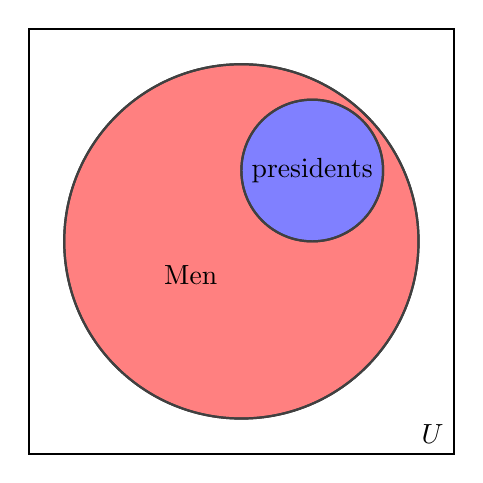
\begin{tikzpicture}[scale=.9]
	\def\circleA{(1,-1) circle (2.5)} %A
	\def\circleB{(0:2) circle (1)} %B

	\colorlet{circle edgeA}{black!75} 
	\colorlet{circle areaA}{red!50}
	\colorlet{circle edgeB}{black!75} 
	\colorlet{circle areaB}{blue!50}

	\tikzset{
		filledA/.style={fill=circle areaA, draw=circle edgeA, thick},
		filledB/.style={fill=circle areaB, draw=circle edgeB, thick},
		outlineA/.style={draw=circle edgeA, thick},
		outlineB/.style={draw=circle edgeB, thick},
	}

	\begin{scope}[fill opacity=1.0]         
			\fill[filledA] \circleA;
			\fill[filledB] \circleB;    
	\end{scope}

	\draw[outlineA] \circleA node[below left= 5pt] {Men}; 
	\draw[outlineB] \circleB node {presidents}; 
	%\node[anchor=south] at (current bounding box.north) {$A \cup B$}; 
	\draw[thick] (-2,-4) rectangle (4,2) node[anchor=south east] at (current bounding box.south east) {$U$};
	%\draw \circleA node[below=30pt,right=0pt] {\footnotesize{\emph{Dr.\,Ashe}}};
\end{tikzpicture} }\only<5-7>{%%%%little circle in big%%%%%
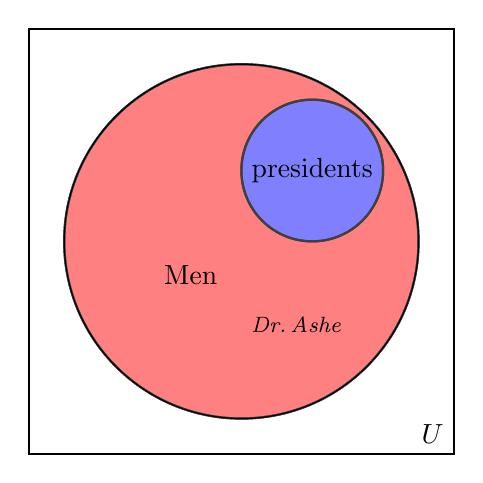
\begin{tikzpicture}[scale=.9]
	\def\circleA{(1,-1) circle (2.5)} %A
	\def\circleB{(0:2) circle (1)} %B

	\colorlet{circle edgeA}{black!75} 
	\colorlet{circle areaA}{red!50}
	\colorlet{circle edgeB}{black!75} 
	\colorlet{circle areaB}{blue!50}

	\tikzset{
		filledA/.style={fill=circle areaA, draw=circle edgeA, thick},
		filledB/.style={fill=circle areaB, draw=circle edgeB, thick},
		outlineA/.style={draw=circle edgeA, thick},
		outlineB/.style={draw=circle edgeB, thick},
	}

	\begin{scope}[fill opacity=1.0]         
			\fill[filledA] \circleA;
			\fill[filledB] \circleB;    
	\end{scope}

	\draw[outlineA] \circleA node[below left= 5pt] {Men}; 
	\draw[outlineB] \circleB node {presidents}; 
	%\node[anchor=south] at (current bounding box.north) {$A \cup B$}; 
	\draw[thick] (-2,-4) rectangle (4,2) node[anchor=south east] at (current bounding box.south east) {$U$};
	\draw \circleA node[below=30pt,right=0pt] {\footnotesize{\emph{Dr.\,Ashe}}};
\end{tikzpicture} }

\only<8>{%%%%little circle in big%%%%%
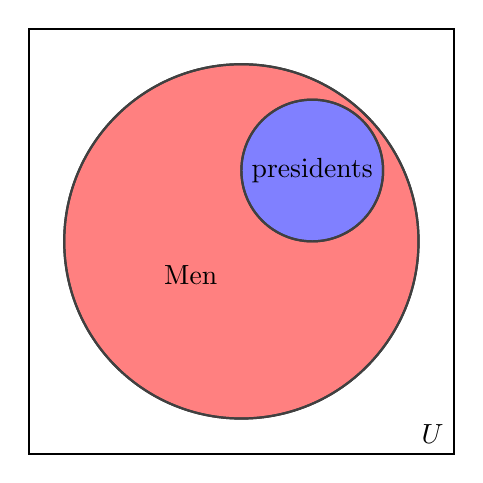
\begin{tikzpicture}[scale=.9]
	\def\circleA{(1,-1) circle (2.5)} %A
	\def\circleB{(0:2) circle (1)} %B

	\colorlet{circle edgeA}{black!75} 
	\colorlet{circle areaA}{red!50}
	\colorlet{circle edgeB}{black!75} 
	\colorlet{circle areaB}{blue!50}

	\tikzset{
		filledA/.style={fill=circle areaA, draw=circle edgeA, thick},
		filledB/.style={fill=circle areaB, draw=circle edgeB, thick},
		outlineA/.style={draw=circle edgeA, thick},
		outlineB/.style={draw=circle edgeB, thick},
	}

	\begin{scope}[fill opacity=1.0]         
			\fill[filledA] \circleA;
			\fill[filledB] \circleB;    
	\end{scope}

	\draw[outlineA] \circleA node[below left= 5pt] {Men}; 
	\draw[outlineB] \circleB node {presidents}; 
	%\node[anchor=south] at (current bounding box.north) {$A \cup B$}; 
	\draw[thick] (-2,-4) rectangle (4,2) node[anchor=south east] at (current bounding box.south east) {$U$};
	%\draw \circleA node[below=30pt,right=0pt] {\footnotesize{\emph{Dr.\,Ashe}}};
\end{tikzpicture} }\only<9-10>{%%%%little circle in big%%%%%
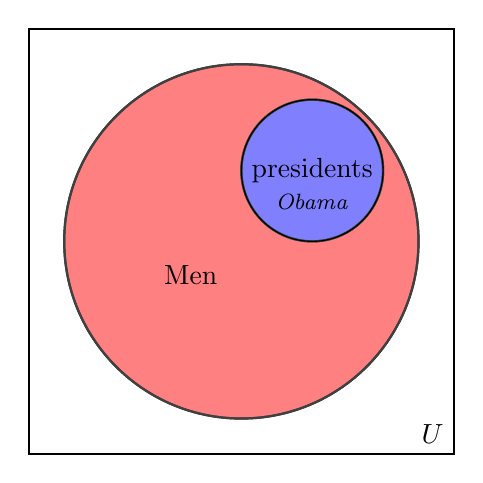
\begin{tikzpicture}[scale=.9]
	\def\circleA{(1,-1) circle (2.5)} %A
	\def\circleB{(0:2) circle (1)} %B

	\colorlet{circle edgeA}{black!75} 
	\colorlet{circle areaA}{red!50}
	\colorlet{circle edgeB}{black!75} 
	\colorlet{circle areaB}{blue!50}

	\tikzset{
		filledA/.style={fill=circle areaA, draw=circle edgeA, thick},
		filledB/.style={fill=circle areaB, draw=circle edgeB, thick},
		outlineA/.style={draw=circle edgeA, thick},
		outlineB/.style={draw=circle edgeB, thick},
	}

	\begin{scope}[fill opacity=1.0]         
			\fill[filledA] \circleA;
			\fill[filledB] \circleB;    
	\end{scope}

	\draw[outlineA] \circleA node[below left= 5pt] {Men}; 
	\draw[outlineB] \circleB node {presidents}; 
	%\node[anchor=south] at (current bounding box.north) {$A \cup B$}; 
	\draw[thick] (-2,-4) rectangle (4,2) node[anchor=south east] at (current bounding box.south east) {$U$};
	\draw \circleB node[below=5pt] {\footnotesize{\emph{Obama}}};
\end{tikzpicture} }

\only<11>{%%%%little circle in big%%%%%
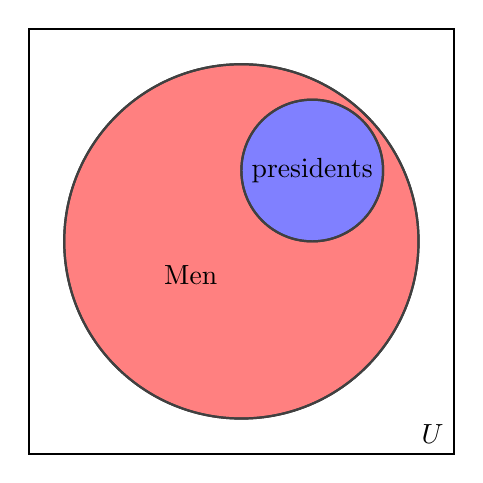
\begin{tikzpicture}[scale=.9]
	\def\circleA{(1,-1) circle (2.5)} %A
	\def\circleB{(0:2) circle (1)} %B

	\colorlet{circle edgeA}{black!75} 
	\colorlet{circle areaA}{red!50}
	\colorlet{circle edgeB}{black!75} 
	\colorlet{circle areaB}{blue!50}

	\tikzset{
		filledA/.style={fill=circle areaA, draw=circle edgeA, thick},
		filledB/.style={fill=circle areaB, draw=circle edgeB, thick},
		outlineA/.style={draw=circle edgeA, thick},
		outlineB/.style={draw=circle edgeB, thick},
	}

	\begin{scope}[fill opacity=1.0]         
			\fill[filledA] \circleA;
			\fill[filledB] \circleB;    
	\end{scope}

	\draw[outlineA] \circleA node[below left= 5pt] {Men}; 
	\draw[outlineB] \circleB node {presidents}; 
	%\node[anchor=south] at (current bounding box.north) {$A \cup B$}; 
	\draw[thick] (-2,-4) rectangle (4,2) node[anchor=south east] at (current bounding box.south east) {$U$};
	%\draw \circleA node[below=30pt,right=0pt] {\footnotesize{\emph{Dr.\,Ashe}}};
\end{tikzpicture} }\only<12-13>{%%%%little circle in big%%%%%
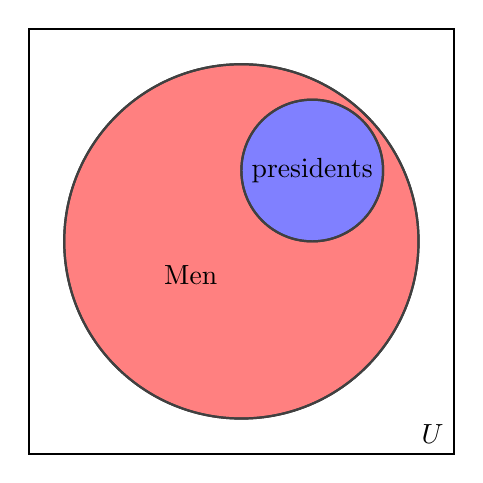
\begin{tikzpicture}[scale=.9]
	\def\circleA{(1,-1) circle (2.5)} %A
	\def\circleB{(0:2) circle (1)} %B

	\colorlet{circle edgeA}{black!75} 
	\colorlet{circle areaA}{red!50}
	\colorlet{circle edgeB}{black!75} 
	\colorlet{circle areaB}{blue!50}

	\tikzset{
		filledA/.style={fill=circle areaA, draw=circle edgeA, thick},
		filledB/.style={fill=circle areaB, draw=circle edgeB, thick},
		outlineA/.style={draw=circle edgeA, thick},
		outlineB/.style={draw=circle edgeB, thick},
	}

	\begin{scope}[fill opacity=1.0]         
			\fill[filledA] \circleA;
			\fill[filledB] \circleB;    
	\end{scope}

	\draw[outlineA] \circleA node[below left= 5pt] {Men}; 
	\draw[outlineB] \circleB node {presidents}; 
	%\node[anchor=south] at (current bounding box.north) {$A \cup B$}; 
	\draw[thick] (-2,-4) rectangle (4,2) node[anchor=south east] at (current bounding box.south east) {$U$};
	%\draw \circleA node[below=30pt,right=0pt] {\footnotesize{\emph{Dr.\,Ashe}}};
\end{tikzpicture} }

\only<7>{\vspace{-.5cm}\textbf{Invalid Argument}
\begin{itemize}
\item $Men\nsubseteq presidents$
\item $\mbox{Dr.\,\ Ashe}\in Men\nRightarrow\mbox{Dr.\,\ Ashe}\notin president$
\end{itemize}
}

\only<10>{\vspace{-.5cm}\textbf{Invalid Argument}
\begin{itemize}
\item $Men\nsubseteq presidents$
\item $x\in Men\nRightarrow x\notin president$
\end{itemize}
}

\only<14>{\vspace{-.5cm}\textbf{Valid Argument}
\begin{itemize}
\item $presidents\subseteq Men$
\item $x\in presidents\Rightarrow x\in Men$
\end{itemize}
}
\end{columns}
\end{frame}

\begin{frame}{Problems}

\prob{1}{1}{Construct a Venn diagram to determine the validity of the argument}{
\begin{enumerate}
\item [1.]All Olympic gold medalists are role models.
\item [2.]Michael Phelps is a role model.
\end{enumerate}
\vspace{-10pt} \rule[0.25ex]{1\columnwidth}{1pt}
\begin{itemize}
\item [] \vspace{-15pt}Therefore, Michael Phelps is a gold medalist.
\end{itemize}
}

\prob{2}{2}{Construct a Venn diagram to determine the validity of the argument}{
\begin{enumerate}
\item [1.]All Olympic gold medalists are role models.
\item [2.]Michael Phelps is an Olympic gold medalist.
\end{enumerate}
\vspace{-10pt} \rule[0.25ex]{1\columnwidth}{1pt}
\begin{itemize}
\item [] \vspace{-15pt}Therefore, Michael Phelps is a role model.
\end{itemize}
}

\prob{3}{3}{Construct a Venn diagram to determine the validity of the argument}{
\begin{enumerate}
\item [1.]All professional wrestlers are actors.
\item [2.]Ralph Nader is not an actor.
\end{enumerate}
\vspace{-10pt} \rule[0.25ex]{1\columnwidth}{1pt}
\begin{itemize}
\item [] \vspace{-15pt}Therefore, Ralph Nader is not a professional wrestler.
\end{itemize}
}

\prob{4}{4}{Construct a Venn diagram to determine the validity of the argument}{
\begin{enumerate}
\item [1.]All professional wrestlers are actors.
\item [2.]Ralph Nader is not a professional wrestler.
\end{enumerate}
\vspace{-10pt} \rule[0.25ex]{1\columnwidth}{1pt}
\begin{itemize}
\item [] \vspace{-15pt}Therefore, Ralph Nader is not an actor.
\end{itemize}
}

\prob{5}{5}{Construct a Venn diagram to determine the validity of the argument}{
\begin{enumerate}
\item [1.]All professional wrestlers are actors.
\item [2.]''The Rock'' is not a professional wrestler.
\end{enumerate}
\vspace{-10pt} \rule[0.25ex]{1\columnwidth}{1pt}
\begin{itemize}
\item [] \vspace{-15pt}Therefore, ``The Rock'' is not an actor.
\end{itemize}
}
\end{frame}

\begin{frame}{Inductive Arguments}

\vspace{-.5cm}
\begin{columns}


\column{5.5cm}
\begin{block}<5->{}
The conclusion in an inductive argument \emph{is never guaranteed}.\emph{ }
\end{block}

\column{5.5cm}
\begin{exampleblock}{Example}
What comes next? 
\[
2,4,6,8,10,12,\underline{\,\,\,\,\,\,\,\,\,}
\]

\begin{itemize}
\item <2->if the numbers are integers.
\item <3->if the numbers are on a clock.
\item <4->if we count by $2$ except every \nth{7} place is $\smiley$. 
\end{itemize}
\end{exampleblock}
\end{columns}
\prob{6}{6}{Fill in the blank with what is \emph{most likely} to be the next. Explain the pattern generated by your answer.}{
\[
0,5,10,15,20,\dots
\]
}

\prob{7}{7}{Fill in the blank with what is \emph{most likely} to be the next. Explain the pattern generated by your answer.}{
\[
0,2,6,12,20,\dots
\]
}

\prob{8}{8}{Fill in the blank with what is \emph{most likely} to be the next. Explain the pattern generated by your answer.}{
\[
1,1,2,3,5,\dots
\]
}

\prob{9}{9}{Fill in the blank with what is \emph{most likely} to be the next. Explain the pattern generated by your answer.}{
\[
2,3,5,7,11,\dots
\]
}
\end{frame}

\end{document}
